% Mirror: https://github.com/SIGma-UIUC/presentation-format
% --------------------------------------------------------------------
% This is a simple Beamer document that uses beamerthemesigma.sty
% Reading the comments should help you create a presentation even if
% you've never used Beamer before.
% --------------------------------------------------------------------

% Set our document class to Beamer
\documentclass[aspectratio=169]{beamer}
% \documentclass[aspectratio=169, handout]{beamer}
% Add handout option to ignore pauses

% From Jeff E
\usepackage{algo}
% Some more macros
\usepackage{sigmastyle}


% Set a title
\title{Kolmogorov Complexity}

% Set a subtitle if you desire
%\subtitle{[TAOCP 5 8.9.10.11]}

% Whoever worked on the presentation:
\author{Eyad Loutfi}

% Date looks ugly, so leave blank
\date{}

% An institute name, if you're so inclined
% \institute{University of Illinois Urbana-Champaign}

% Use the SIGma theme for this Beamer presentation
\usetheme{sigma}
% --------------------------------------------------------------------

% Begin document
\begin{document}

% Beamer calls each slide a "frame", defined within the environment:
% \begin{frame}
%   <frame content here>
% \end{frame}

% This frame is just the title.
\begin{frame}
\titlepage
\end{frame}

\section{Basics}
% Section pages can be printed thus:
\frame{\sectionpage}

\begin{frame}{Computability}
  
  \begin{itemize}
    \item A program is something that takes in a string as input and has one as output, all within some model of computation -- more on this in a bit. \pause
    \item A natural question to ask is if there is a correspondence between strings and the programs that output them. \pause
    \item To what extent might a ``large'' string be produced by a ``short'' program, i.e. how much might we be able to ``compress'' strings?
  \end{itemize}
\end{frame}

\begin{frame}{Turing Machines}
  
  \begin{itemize}
    \item First we need to introduce models of computation. The classic model of computation is the \emph{Turing machine}. \pause
    \item TM's are defined over a finite alphabet, have an infinite tape that has the input at the start of it, a read head with internal state that starts at the start of the tape and can write or move left or right all according to some finite instructions (transition function based on the head's state and character in the cell it's over). 
  \end{itemize}
  \begin{center}
    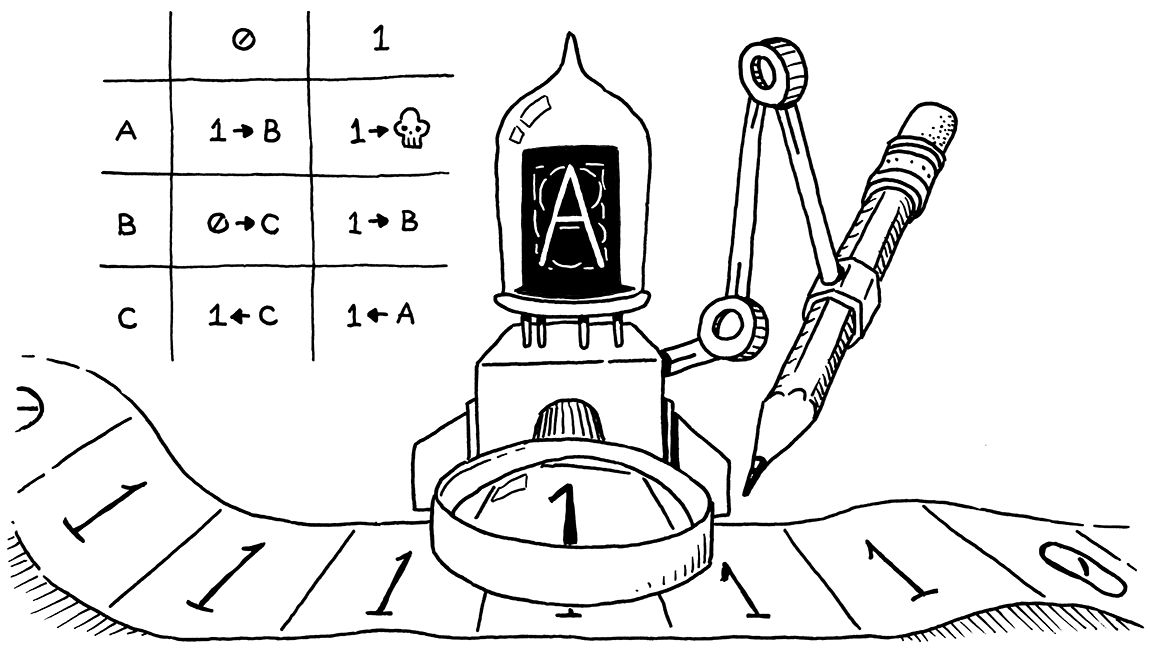
\includegraphics[width=0.5\textwidth, height=0.5\textheight, keepaspectratio]{Turing_pic.png}
  \end{center}
\end{frame}

\begin{frame}{Computability}
  
  \begin{itemize}
    \item This turns out to be as powerful as any computer we know! The \emph{Church Turing} thesis states that anything a computer can do can be done by a Turing machine. \pause
    \item When we say model of computation, we mean anything that can represent all the functions a computer can, which all your favorite programming languages (C, Python) can do since they're Turing Complete (can do anything a Turing machine can). \pause
    \item Note that programs/TM's etc are defined by precise descriptions, so in a sense they are strings themselves! \pause
    \item One can devise an encoding scheme of all programs -- many such encodings exist, could use all binary strings or all ASCII strings, etc.
  \end{itemize}
\end{frame}

\begin{frame}{Computability}
  
  \begin{itemize}
    \item More importantly, the encoding is done in such a way that a program can recognize it -- such that we can define a program to simulate the behavior of a machine as a result of parsing the encoding. \pause
    \item This means we can define a program to be able to simulate any other program -- a very important result! \pause
    \item Other important definitions: A set is ``recursively enumerable,'' or RE if there exists a program that can give a ``yes'' answer to any string in the set. A set is ``computable'' if a program like that exists that also gives a ``no'' answer for any string not in the set. \pause
    \item These properties are not guaranteed in general due to possibility of infinite looping.
  \end{itemize}
\end{frame}


\begin{frame}{Kolmogorov Complexity}
  
  \begin{itemize}
    \item Intuitively, 057835292 has the same probability of being selected as 000000000, yet one of these feels more ``complex'' to us. \pause
    \item Solution: We define the complexity of a string be the length of the shortest program that prints it. This is \emph{Kolmogorov complexity}. \pause
    \item Limitation: Must be relative to a model of computation / programming language you fix. \pause
    \item Gives us a powerful tool for understanding compression, the distribution of ``complexity'' among finite strings themselves, and even limitative results of mathematics as a whole.
  \end{itemize}
\end{frame}

% Start a section: *sections* (subsections, etc.) are what show up in the TOC.
\section{Some Fundamental Proofs}
% Section pages can be printed thus:
\frame{\sectionpage}
% There's a way to automate this, see:
% https://tex.stackexchange.com/questions/178800/creating-sections-each-with-title-pages-in-beamers-slides/178803

\begin{frame}{Invariance Theorem}
  
  \begin{itemize}
    \item It might seem like we are completely limited talking about Kolmogorov complexity across languages since it is relative to them. \pause
    \item Rather, the K complexity only differs by a constant factor between different languages.
  \end{itemize}
\end{frame}

\begin{frame}
  % Alternate syntax for frame titles
  \frametitle{Invariance Theorem}
  % Frames can have subtitles:
  % Some frame content:
  \begin{thrm}
    Given $2$ languages $L_1, L_2$ and their respective K complexities $K_1, K_2$, for any string $s$, $K_1(s) \leq K_2(s) + c$ for some constant $c$.
  \end{thrm}
  \pause
  \begin{pf}
    \begin{enumerate}
        \item Suppose we have an interpreter in $L_1$ for strings $p$ representing programs in $L_2$, $Interpret(p)$, meaning it will produce the output that $p$ would have produced in $L_2$. \pause
        \item Let $P$ be the shortest program in $L_2$ that outputs $s$. \pause
        \item Then $Interpret(P)$ will produce $s$ in $L_1$. \pause
        \item We know $|Interpret(P)| = |Interpret| + |P|$, but $|P| = K_2(s)$ and we can consider $|Interpret|$ to be some constant $c$. \pause
        \item Therefore $K_1(s) \leq K_2(s) + c$.
    \end{enumerate}
  \end{pf}
\end{frame}

% Use \pause to make stuff readable
% Large walls of text scare the audience, we don't want that
% Introducing stuff sequentially allows for questions
\begin{frame}
  % Alternate syntax for frame titles
  \frametitle{Universal Lossless Compression}
  % Frames can have subtitles:
  % Some frame content:
  \begin{thrm}
    For every $n$, there exists a length $n$ string $a$ whose Kolmogorov complexity $K(a)$ is at least $n$.
  \end{thrm}
  \pause
  \begin{pf}
    \begin{enumerate}
        \item Suppose for contradiction that every string $a$ in $\{0, 1\}^n$, of which there are $2^n$ of, $K(a) < n$. \pause
        \item Then we have a one-to-one function $f$, such that $f(a)$ will output the string representing the shortest program that outputs $a$. \pause
        \item Number of shorter strings is 
        $\sum_{i=0}^{n-1}\abs{\{0,1\}^i} = 1 + 2 + 2^2 + ... + 2^{n-1} = 2^n-1$ \pause
        \item For $f$ to be one-to-one, there would have be $\geq 2^n$ output programs but we only have $2^n - 1$. Contradiction
    \end{enumerate}
  \end{pf}
\end{frame}


\begin{frame}{Universal Lossless Compression}
    \begin{itemize}
        \item What this tells us is there will always be incompressible strings where $K(a) \geq \abs{a}$, i.e. universal lossless compression is impossible! \pause
        \item We can now prove an even more general fact regarding the computability of $K$!
    \end{itemize}
\end{frame}

\begin{frame}
  % Alternate syntax for frame titles
  \frametitle{Uncomputability of K}
  % Frames can have subtitles:
  % Some frame content:
  \framesubtitle{The proof uses the fact programs can simulate other programs and that there is a binary string encoding scheme for all programs}
  \begin{thrm}
    There is no possible program $P(x, i)$ that outputs ``yes'' if $K(x) = i$ and ``no'' if $K(x) \neq i$.
  \end{thrm}
  \pause
  \begin{pf}
    \begin{itemize}
        \item Suppose there is such a program $P$. We construct another program $\textsc{Q}(j)$ as follows: \pause
        \begin{algo}
        \underline{\textsc{Q}$(j)$}:\+
        \\ for each binary string encoding $x$ of a program \+
        \\  Simulate $P(x, j)$
        \\ If simulation outputs ``yes'' \+
        \\      print $x$ \Comment{This will be the first program $x$ s.t. $K(x) = j$} \- \-
        \end{algo}
    \end{itemize}
  \end{pf}
\end{frame}

\begin{frame}
  % Alternate syntax for frame titles
  \frametitle{Uncomputability of K Continued}
  % Frames can have subtitles:
  % Some frame content:
  \begin{pf}
    \begin{itemize}
        \item Let $y$ be the output of $Q(j)$. \pause
        \item Therefore $P(y, j)$ outputs ``yes'', which implies $K(y) = j$ \pause
        \item Since $Q(j)$ is a program that outputs $y$, the length of $Q(j)$ must be at least $j$. \pause
        \item We know $Q(j)$ includes $P$ in it's definition, in addition to needing to write the input $j$, so $|Q(j)| = |P| + |j| + c$ where $c$ is some constant overhead by $P$. \pause
        \item We need at most $\log(j)$ bits to write $j$, so we obtain the inequality $K(y) = j \leq |Q(j)| \leq |P| + \log(j) + c \Rightarrow j - \log(j) \leq |P| + c$ \pause
        \item This will be true no matter what $j$ we pick, yet since $j - \log(j)$ is unbounded and $P$ and $c$ are fixed, there will be a $j$ that makes it greater than $|P| + c$, a contradiction. \pause
        \item Therefore Kolmogorov complexity is not computable, there cannot exist such a program $P$.
    \end{itemize}
  \end{pf}
\end{frame}

\section{What we can say about the complexity of strings?}
% Section pages can be printed thus:
\frame{\sectionpage}

\begin{frame}{Average Complexity of Finite Strings}
  
  \begin{itemize}
    \item A natural question to ask is what the distribution of Kolmogorov complexity over the average binary string really looks like \pause
    \item Intuitively we would expect most strings to appear random, and it turns out this intution is true: The vast majority of strings are not very compressible. 
  \end{itemize}
\end{frame}

\begin{frame}
  % Alternate syntax for frame titles
  \frametitle{Average Complexity of Finite Strings}
  % Frames can have subtitles:
  % Some frame content:
  \begin{thrm}
    If $A$ is the set of all strings $a$ where $K(a) < n - k$, then $\frac{|A|}{|\{0, 1\}^n|} < \frac{1}{2^k}$ 
  \end{thrm}
  \pause
  \begin{pf}
    \begin{enumerate}
        \item There is a one-to-one function from $A$ to the set $C$ of all binary strings with length less than $n - k$.
        \begin{itemize}
            \item $\abs{C} = 2^{n - k} - 1$
        \end{itemize} \pause
        \item So $|A| \leq |C| = 2^{n-k}-1 \Rightarrow |A| < 2^{n-k}$. \pause
        \item Therefore $\frac{|A|}{|\{0,1\}^n|} < \frac{2^{n-k}}{2^n} = \frac{1}{2^k}$. 
    \end{enumerate}
  \end{pf}
\end{frame}

\begin{frame}{Average Complexity of Finite Strings}
  
  \begin{itemize}
    \item This implies the proportion of binary strings that can be compressed to be 2 bits shorter is less than a half, the ones that can be compressed to be 3 bits shorter is less than a quarter. \pause
    \item When looking at strings of length 100, the proportion of them that can be compressed to be even just 10 bits less is less than $\frac{1}{2^9}$, or less than about $0.2\%$ \pause
    \item Not only are most strings hard to compress, but we can actually prove an upper bound on the Kolmogorov complexity that we are even able to PROVE a string to have.
  \end{itemize}
\end{frame}

\begin{frame}{Proof System}
  
  \begin{itemize}
    \item Before we continue, we'll introduce the notion of a \emph{proof system}. \pause
    \item A proof system is defined via
    \begin{itemize}
        \item A computable language (set of strings) which we'll usually take to be well formed formulas expressed in some logic \pause
        \item A distinguished RE subset of that language we call the \emph{axioms}
        \item A set of \emph{theorems} that include the axioms. \pause
        \item A set of inference rules that can be programmed and can be applied to any theorem to create other theorems.
    \end{itemize}
    The set of all theorems that can be produced this way is then called the proof system. \pause
    \item Intuitively this is just a model of how we prove things, but the key insight is we only ever do proofs using computable inference rules.
  \end{itemize}
\end{frame}

\begin{frame}{Example Inference Rules in First Order Logic}
\begin{itemize}
    \item Clearly proof systems are RE -- one can just make a program that starts at the axioms and repeatedly apply the inference rules -- like these from first order logic. 
  \end{itemize}
  \begin{center}
    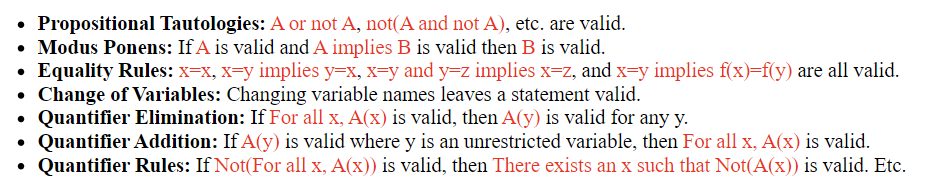
\includegraphics[width=1\textwidth]{Exinference.png}
  \end{center}
  
\end{frame}

\begin{frame}{Math is Incomplete}
\begin{itemize}
    \item One result that immediately follows from the uncomputability of $K$ is Godel's First Incompleteness theorem, that any RE proof system for mathematics will not be able prove or disprove every statement in the language associated with it. 
    \item This is because if we could, then the fact the proof system is RE implies we can have a program loop through all theorems till it finds the statement for what the Kolmogorov complexity of a string is or isn't for any string, which would make $K$ computable which we already proved is impossible. \pause
    \item Godel's result was more powerful, applying to any system that can prove facts regarding basic arithmetic, though this still applies since logical statements about programs may be encoded as arithmetical statements -- i.e. Godel numbering.
  \end{itemize}
  
\end{frame}

\begin{frame}{Godel Numbering}
\begin{itemize}
    \item Fundamental Theorem of Arithmetic ensures that any Godel number has a unique prime factorization - allowing one to retrieve the original statement using the prime factors. 
  \end{itemize}
  \begin{center}
    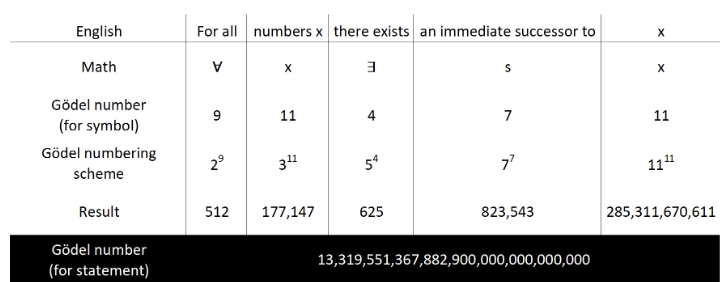
\includegraphics[width=1\textwidth]{ex_encode.PNG}
  \end{center}
  
\end{frame}

\begin{frame}{Chaitin's Incompleteness Theorem}
  
``The proof of this closely resembles G. G. Berry’s paradox of ‘the first natural number which cannot be named in less than a billion words.’ The version of Berry’s paradox that will do the trick is ‘that object having the shortest proof that its algorithmic information content is greater than a billion bits.'' -- Gregory Chaitin

\end{frame}

\begin{frame}{Chaitin's Incompleteness Theorem}
  
  \begin{thrm}
    For any proof system $F$, there is a largest number $L$ such that $F$ cannot prove that the Kolmogorov complexity of any bit string is more than $L$. 
  \end{thrm} \pause
  \begin{itemize}
    \item Suppose not, so there is some RE system $F$ such that for any $L$, $F$ can prove $K(x) = L$ for some $x$. \pause
    \item We construct a program $P$ that takes in an integer $L$ and iterates through all proofs in $F$ until it finds a proof of $K(x) = L$ for some $x$, then prints that $x$.
  \end{itemize}
\end{frame}

\begin{frame}{Chaitin's Incompleteness Theorem Continued}
  
  \begin{itemize}
    \item Let $x$ be the output of $P$ for a certain $L$, therefore $K(x) = L$, and since $P(L)$ outputs $x$, $L \leq P(L) = |P| + |L| + c \leq |P| + \log(L) + c$ where $c$ is some constant overhead by $P$. \pause
    \item This means regardless of $L$, $L - \log(L) \leq |P| + c$, but since $P$ and $c$ are fixed, for large enough $L$ this will clearly not hold. \pause
    \item Therefore for any such proof system $F$, there must exist an $L$ such that no string can be proven to have Kolmogorov complexity of $L$, or any number bigger since it will still violate the inequality. 
  \end{itemize}
\end{frame}

\begin{frame}{Chaitin's Incompleteness Theorem Continued}
  
  \begin{itemize}
    \item This further implies any program that would take in an input and calculate a lower bound on it's Kolmogorov complexity cannot exceed some limit. 
  \end{itemize}
  \begin{center}
    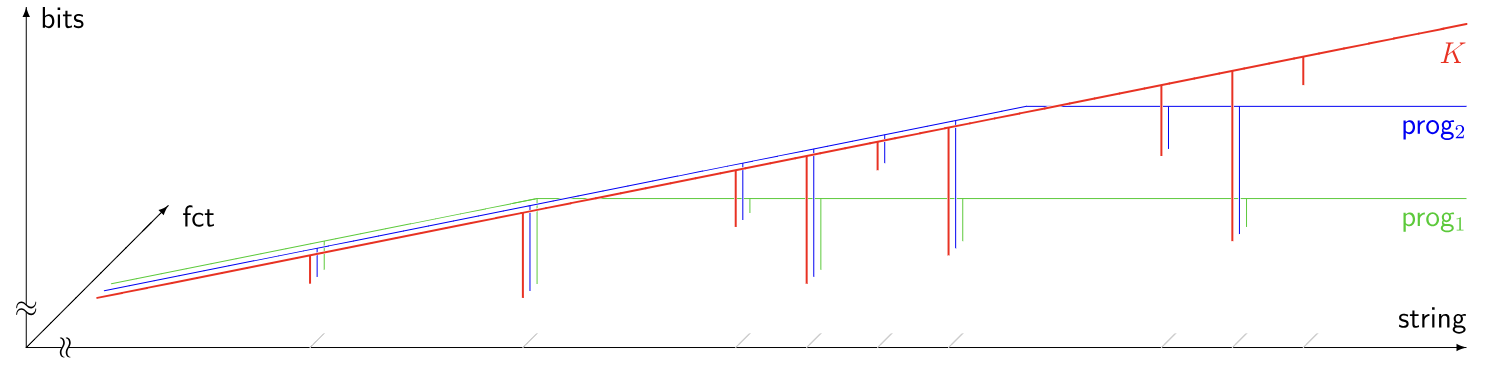
\includegraphics[width=1\textwidth]{K_C_ex.png}
  \end{center}
\end{frame}

\begin{frame}{The End}

  \begin{center}
    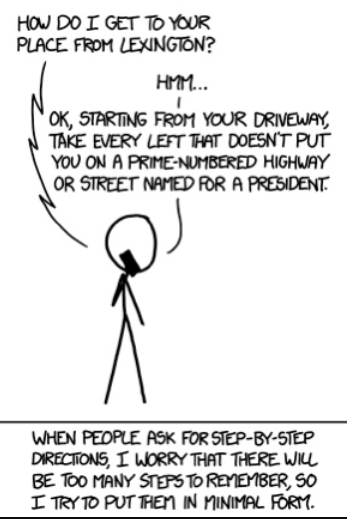
\includegraphics[width=0.4\textwidth]{meme.png}
  \end{center}
\end{frame}


\end{document}